\section{Evaluation}
\label{sec:evaluation}

\subsection{Measurement of heat capacity $C_p$}
To determine the heat capacity at constant pressure $C_p$, the resistance $R$, voltage $U$, current $I$ and time $t$ are measured.
Uncertainties are estimated for the quantities:
\begin{align*}
    \sigma_R &= \qty{0.1}{\ohm} \\
    \sigma_U &= \qty{0.01}{\volt}\\
    \sigma_I &= \qty{0.1}{\milli\ampere} \\
    \sigma_t &= \qty{5}{\second}
\end{align*}
The reason for this is that the measuring instruments have a limited resolution.
In the following calculations, the error propagation is calculated using the Python library \textbf{Uncertainties} \cite{uncertainties}.
\\
The supplied energy in the time period $\Delta t$
\begin{equation}
    \Delta E = U \cdot I \cdot \Delta t \, .
\end{equation}
can be used to determine the molar heat capacity
\begin{equation}
    C_p = \frac{\Delta E}{\Delta T} \frac{M}{m} \,.
\end{equation}
The mass of the copper sample $m = \qty{342}{\gram}$ \cite{V47} and the molar mass of copper $M = \qty{63.5}{\frac{\gram}{\mol}}$ \cite{goodfellow} are used for this.
All measured values and the determined heat capacities are listed in \autoref{tab:C_p}.
The temperature dependency of the heat capacity $C_p$ is shown in \autoref{fig:C_p}.
Also marked is the theoretical value of the Dulong–Petit law according to \autoref{eq:dulong}.
\begin{table}
    \centering
    \caption{The temperature difference $\Delta T$ of the sample in the time period $t$ with the current $I$ applied at voltage $U$. The resulting heat capacity at constant pressure is denoted as $C_p$.}
    \label{tab:C_p}
    \begin{tabular}{c c c c c}
        \toprule
        $\Delta T \,/\, \unit{\kelvin}$ & $U \,/\, \unit{\volt}$ & $I \,/\, \unit{\milli\ampere}$ & $\Delta t \,/\, \unit{\second}$ & $C_p \,/\, \unit{\frac{\joule}{\mol \cdot \kelvin}}$ \\
        \midrule
        $2.13\pm0.33$ & $16.150\pm0.010$ & $153.20\pm0.10$ & $105\pm7$ & $24\pm4$ \\
        $9.26\pm0.34$ & $16.310\pm0.010$ & $154.70\pm0.10$ & $349\pm7$ & $18.6\pm0.8$ \\
        $10.02\pm0.34$ & $16.310\pm0.010$ & $154.70\pm0.10$ & $391\pm7$ & $19.3\pm0.7$ \\
        $9.83\pm0.34$ & $16.790\pm0.010$ & $159.00\pm0.10$ & $323\pm7$ & $17.2\pm0.7$ \\
        $10.11\pm0.34$ & $19.000\pm0.010$ & $181.00\pm0.10$ & $296\pm7$ & $19.7\pm0.8$ \\
        $9.92\pm0.34$ & $19.050\pm0.010$ & $181.00\pm0.10$ & $343\pm7$ & $23.4\pm0.9$ \\
        $9.96\pm0.34$ & $17.180\pm0.010$ & $162.80\pm0.10$ & $470\pm7$ & $25.9\pm1.0$ \\
        $10.01\pm0.35$ & $17.260\pm0.010$ & $163.40\pm0.10$ & $425\pm7$ & $23.5\pm0.9$ \\
        $10.05\pm0.35$ & $17.300\pm0.010$ & $163.70\pm0.10$ & $448\pm7$ & $24.7\pm0.9$ \\
        $10.10\pm0.35$ & $17.330\pm0.010$ & $163.90\pm0.10$ & $470\pm7$ & $25.9\pm1.0$ \\
        $9.89\pm0.35$ & $17.350\pm0.010$ & $164.10\pm0.10$ & $415\pm7$ & $23.4\pm0.9$ \\
        $9.94\pm0.35$ & $17.360\pm0.010$ & $164.20\pm0.10$ & $437\pm7$ & $24.6\pm1.0$ \\
        $9.98\pm0.35$ & $17.380\pm0.010$ & $164.30\pm0.10$ & $438\pm7$ & $24.6\pm1.0$ \\
        $10.02\pm0.35$ & $17.380\pm0.010$ & $164.40\pm0.10$ & $450\pm7$ & $25.1\pm1.0$ \\
        $9.80\pm0.4$ & $17.390\pm0.010$ & $164.50\pm0.10$ & $457\pm7$ & $26.1\pm1.0$ \\
        $10.1\pm0.4$ & $17.390\pm0.010$ & $164.60\pm0.10$ & $463\pm7$ & $25.7\pm1.0$ \\
        $9.9\pm0.4$ & $17.400\pm0.010$ & $164.70\pm0.10$ & $425\pm7$ & $24.1\pm1.0$ \\
        $10.2\pm0.4$ & $17.400\pm0.010$ & $164.80\pm0.10$ & $495\pm7$ & $27.3\pm1.0$ \\
        $10.0\pm0.4$ & $17.400\pm0.010$ & $164.80\pm0.10$ & $460\pm7$ & $25.9\pm1.0$ \\
        $10.0\pm0.4$ & $17.390\pm0.010$ & $164.80\pm0.10$ & $470\pm7$ & $26.3\pm1.0$ \\
        $10.1\pm0.4$ & $17.390\pm0.010$ & $164.90\pm0.10$ & $500\pm7$ & $27.9\pm1.1$ \\
        $10.1\pm0.4$ & $17.390\pm0.010$ & $164.90\pm0.10$ & $500\pm7$ & $27.8\pm1.1$ \\
        $9.9\pm0.4$ & $17.380\pm0.010$ & $165.00\pm0.10$ & $460\pm7$ & $26.2\pm1.1$ \\
        \bottomrule
    \end{tabular}
\end{table}
\begin{figure}
    \centering
    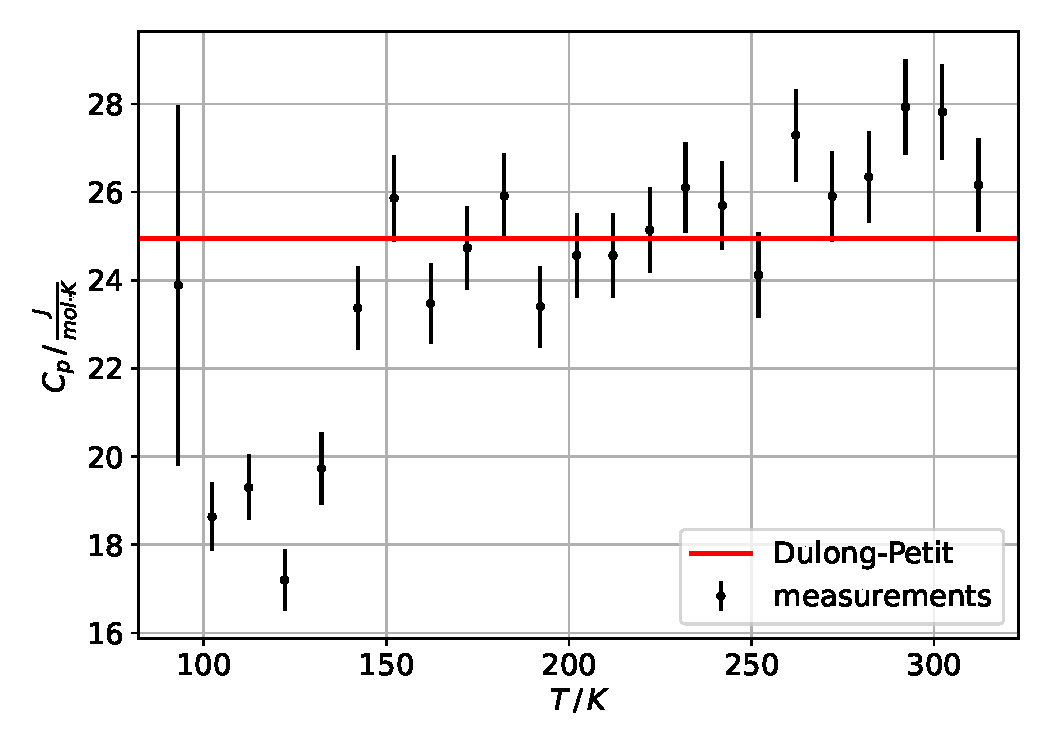
\includegraphics[width=0.8\textwidth]{content/plots/C_p.pdf}
    \caption{The measured temperature dependency of the heat capacity at constant pressure $C_p$.
    The red line represents the theoretical value for the classical Debye model $C = 3 \cdot R = \qty{24.9}{\frac{\joule}{\mol \cdot \kelvin}}$, where $R$ is the general gas constant.}
    \label{fig:C_p}
\end{figure}
\FloatBarrier

\subsection{Heat capacity at constant volume $C_V$}
The relation between the measured heat capacity at constant pressure $C_p$ and the heat capacity at constant volume $C_V$ is given by  %!REF
\begin{equation}
        C_p - C_V = 9 \cdot \alpha^2 \cdot \kappa \cdot V_0 \cdot T \, ,
        \label{eqn:C_relation}
\end{equation}
where $\alpha$ is the thermal expansion, $\kappa$ the bulk modulus and $V_0 = \frac{M}{\rho}$ the molar volume with the density of cupper $\rho$.
The values of this parameters $\kappa = \qty{137.8}{\giga\pascal}$ and $\rho = \qty{8960}{\frac{\kilogram}{\metre^3}}$ are taken from source \cite{goodfellow}.
The thermal expansion depends on the temperature and shows a $\frac{1}{T}$ behavior
\begin{equation}
    \alpha = a_1 \cdot \frac{1}{T} + a_2 \, .
\end{equation}
A fit with the non-linear least squares method is performed with the python library Scipy\cite{scipy} on the given value pairs ($T, \alpha$) \cite{V47}.
The fitted function with the parameters
\begin{align*}
    a_1 &= \qty{-8.73(4)e-04}{} \\
    a_2 &= \qty{1.9411(29)e-05}{\frac{1}{\kelvin}}
\end{align*}
is shown in \autoref{fig:alpha}.
\begin{figure}
    \centering
    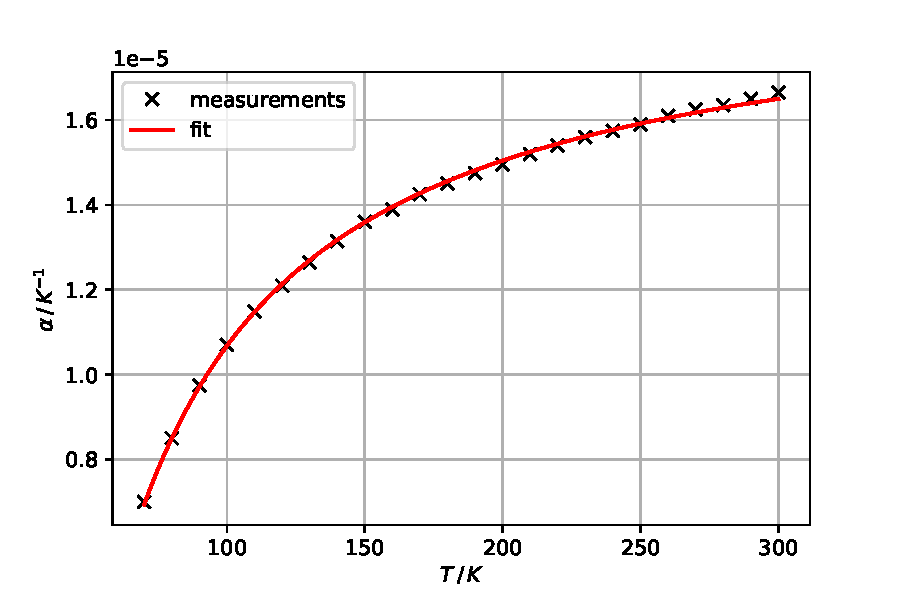
\includegraphics[width=0.8\textwidth]{content/plots/temperature_progress.pdf}
    \caption{The fitted temperature dependence of $\alpha$ and the given values.}
    \label{fig:alpha}
\end{figure}
The function returns the thermal expansion $\alpha$ at the measured temperature $T$.
The heat capacity $C_V$ is now calculated with \autoref{eqn:C_relation} and can be viewed in \autoref{fig:C_v}.
The numerical values of $\alpha$ and $C_V$ are listed in \autoref{tab:C_v}.
\begin{figure}
    \centering
    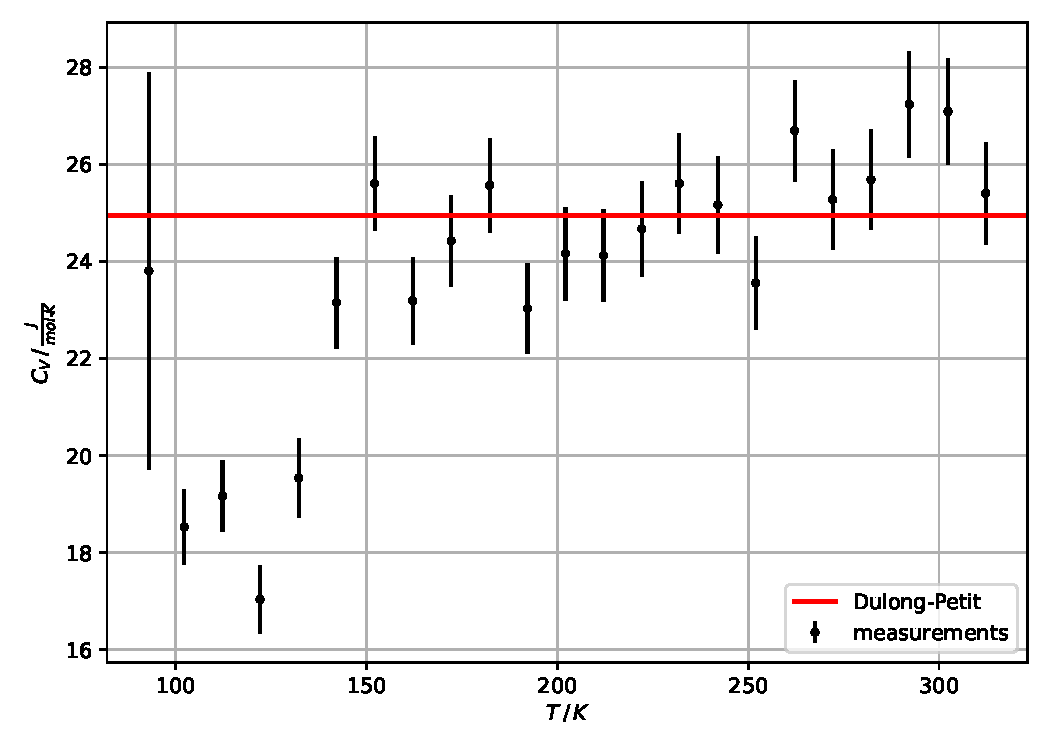
\includegraphics[width=0.8\textwidth]{content/plots/C_v.pdf}
    \caption{The resulting temperature dependency of the heat capacity at constant volume $C_v$.
    The red line represents the theoretical value for the classical Debye model $C = 3 \cdot R = \qty{24.9}{\frac{\joule}{\mol \cdot \kelvin}}$, where $R$ is the general gas constant.
    }
    \label{fig:C_v}
\end{figure}
\begin{table}
    \centering
    \caption{The thermal expansion $\alpha$ resulting from the fit for the temperature $T$, the measured heat capacity at constant pressure $C_p$ and the determined heat capacity at constant volume.}
    \label{tab:C_v}
    \begin{tabular}{c c c c}
        \toprule
        $T \,/\, \unit{\kelvin}$ & $C_p \,/\, \unit{\frac{\joule}{\mol \cdot \kelvin}}$ & $\alpha \cdot 10^{-5} \,/\, \unit{\kelvin^{-1}}$ & $C_v \,/\, \unit{\frac{\joule}{\mol \cdot \kelvin}}$\\
        \midrule
        $93.05\pm0.24$ & $24\pm4$ & $1.003\pm0.006$ & $24\pm4$ \\
        $102.31\pm0.24$ & $18.6\pm0.8$ & $1.088\pm0.005$ & $18.5\pm0.8$ \\
        $112.33\pm0.24$ & $19.3\pm0.7$ & $1.164\pm0.005$ & $19.2\pm0.7$ \\
        $122.15\pm0.24$ & $17.2\pm0.7$ & $1.226\pm0.005$ & $17.0\pm0.7$ \\
        $132.27\pm0.24$ & $19.7\pm0.8$ & $1.281\pm0.004$ & $19.5\pm0.8$ \\
        $142.18\pm0.24$ & $23.4\pm0.9$ & $1.327\pm0.004$ & $23.2\pm0.9$ \\
        $152.15\pm0.24$ & $25.9\pm1.0$ & $1.367\pm0.004$ & $25.6\pm1.0$ \\
        $162.15\pm0.24$ & $23.5\pm0.9$ & $1.403\pm0.004$ & $23.2\pm0.9$ \\
        $172.21\pm0.25$ & $24.7\pm0.9$ & $1.434\pm0.004$ & $24.4\pm0.9$ \\
        $182.30\pm0.25$ & $25.9\pm1.0$ & $1.462\pm0.004$ & $25.6\pm1.0$ \\
        $192.20\pm0.25$ & $23.4\pm0.9$ & $1.487\pm0.004$ & $23.0\pm0.9$ \\
        $202.14\pm0.25$ & $24.6\pm1.0$ & $1.509\pm0.004$ & $24.2\pm1.0$ \\
        $212.12\pm0.25$ & $24.6\pm1.0$ & $1.5296\pm0.0035$ & $24.1\pm1.0$ \\
        $222.14\pm0.25$ & $25.1\pm1.0$ & $1.5481\pm0.0035$ & $24.7\pm1.0$ \\
        $231.95\pm0.25$ & $26.1\pm1.0$ & $1.5648\pm0.0035$ & $25.6\pm1.0$ \\
        $242.06\pm0.25$ & $25.7\pm1.0$ & $1.5805\pm0.0034$ & $25.2\pm1.0$ \\
        $251.96\pm0.25$ & $24.1\pm1.0$ & $1.5947\pm0.0034$ & $23.6\pm1.0$ \\
        $262.15\pm0.26$ & $27.3\pm1.0$ & $1.6081\pm0.0033$ & $26.7\pm1.0$ \\
        $272.13\pm0.26$ & $25.9\pm1.0$ & $1.6203\pm0.0033$ & $25.3\pm1.0$ \\
        $282.15\pm0.26$ & $26.3\pm1.0$ & $1.6317\pm0.0033$ & $25.7\pm1.0$ \\
        $292.21\pm0.26$ & $27.9\pm1.1$ & $1.6424\pm0.0033$ & $27.2\pm1.1$ \\
        $302.31\pm0.26$ & $27.8\pm1.1$ & $1.6524\pm0.0032$ & $27.1\pm1.1$ \\
        $312.19\pm0.26$ & $26.2\pm1.1$ & $1.6615\pm0.0032$ & $25.4\pm1.1$ \\
        \bottomrule
    \end{tabular}
\end{table}
\FloatBarrier

\subsection{Debye's temperature \texorpdfstring{$\theta_\text{D}$}{theta}}
For the determination of the material depending parameter \textbf{Debye's temperature $\theta_\text{D}$}, only temperatures below $\qty{170}{\kelvin}$ are considered.
The fraction $\frac{\theta_\text{D}}{T}$ is taken from source \cite{V47} for each measured temperature $T$.
A simple multiplication with the temperature results in Debye's temperature.
\autoref{tab:debye} contains the determined Debye's temperature $\theta_\text{D}$ for each temperature $T$ with the condition $T < \qty{170}{\kelvin}$. 
\begin{table}
    \centering
    \caption{The Debye's temperature $\theta_\text{D}$ resulting from the heat capacity at constant volume $C_v$ and the temperature $T$.}
    \label{tab:debye}
    \begin{tabular}{c c c c}
        \toprule
        $C_v \,/\, \unit{\frac{\joule}{\mol \cdot \kelvin}}$ & $\frac{\theta_\text{D}}{T}$ & $T \,/\, \unit{\kelvin}$ & $\theta_\text{D} \,/\, \unit{\kelvin}$ \\
        \midrule
        $24\pm4$ & $1.0$ & $93.05\pm0.24$ & $93.05\pm0.24$ \\
        $18.5\pm0.8$ & $2.5$ & $102.31\pm0.24$ & $255.8\pm0.6$ \\
        $19.2\pm0.7$ & $2.4$ & $112.33\pm0.24$ & $269.6\pm0.6$ \\
        $17.0\pm0.7$ & $2.9$ & $122.15\pm0.24$ & $354.2\pm0.7$ \\
        $19.5\pm0.8$ & $2.3$ & $132.27\pm0.24$ & $304.2\pm0.6$ \\
        $23.2\pm0.9$ & $1.2$ & $142.18\pm0.24$ & $170.62\pm0.29$ \\
        $25.6\pm1.0$ & $0.0$ & $152.15\pm0.24$ & $0.0\pm0$ \\
        $23.2\pm0.9$ & $1.2$ & $162.15\pm0.24$ & $194.58\pm0.29$ \\
        \bottomrule
    \end{tabular}
\end{table}

\subsection{Theoretical Debye's temperature \texorpdfstring{$\theta_\text{D}$}{theta} and Debye's frequency \texorpdfstring{$\omega_\text{D}$}{theta}}
To compare the experimental Debye's temperature with a theoretical value we determine the Debye's frequency with \autoref{eq:debye_freq}.
With the sound velocities of copper $\nu_\text{long} = \qty{4.70}{\kilo\meter\per\second}$ and $\nu_\text{trans} = \qty{2.26}{\kilo\meter\per\second}$ the Debye's frequency is
\begin{equation}
    \omega_\text{D,th} = \qty{4.35e13}{\hertz}.
\end{equation}
The Debye's temperature $\theta_\text{D}$ can be calculated via \autoref{eq:debye_temp} to
\begin{equation}
    \theta_\text{D,th} = \qty{332.86}{\kelvin}.
\end{equation}
